\section{Test Cases}\label{chap:datasets}

To test the unbinding procedure, the program will be executed on three datasets.
%All of these datasets represent astrophysical structures made of dark matter particles exclusively.  


%=======================
% DICE
%=======================



The first two of these datasets, named ``\dt'' and ``\ds'', contain highly idealistic structures, where the effects of particle unbinding and the determination of the clump's properties can be seen and evaluated more easily.
They are both created with \dice\ \parencite{DICE}, which ``\textit{models initial conditions of idealized galaxies [...]. The code can set up a large number of components modelling distinct parts of the galaxy, and creates 3D distributions of particles}'' \parencite{DICE}.
Each structure is initially generated as an isolated, spherically symmetric halo.
The halos were chosen to follow the Navarro-Frenk-White (NFW) mass profile.
The individual halos are later joined together to create one large structure that contains substructure(s).
All particle masses are set to be identical.
Furthermore, all particles of a clump are set to be energetically bound to the clump, thus satisfying eq. \eqref{eq:boundv}, where the potential $\phi$ is computed the same way as given in eq. \eqref{eq:sol_phi}.


%=======================
% DICE TWO
%=======================

The \dt\ dataset consists of two clumps created this way.
A smaller halo, made of 40'000 particles, is nested within a bigger halo that contains 200'000 particles, so that it represents a subhalo.
Additionally, the subhalo is set to follow a Kepler orbit with respect to the bigger one with the eccentricity $\varepsilon = 0.1$ so that it has a closed orbit.
The initial particle distribution of the two halos is shown in figure \ref{fig:dice_two_origin}.\\
%
The \dt\ dataset will be used to demonstrate the effects of the choice of parameters relevant for the unbinding procedure in chapter \ref{chap:results}, which are the number of mass bins used to compute the potential and the convergence limit $\varepsilon$ for iterative clump properties determination.





\begin{figure}[htbp!]
	\centering
	\minipage[t]{0.497\textwidth}
		\centering
		\fbox{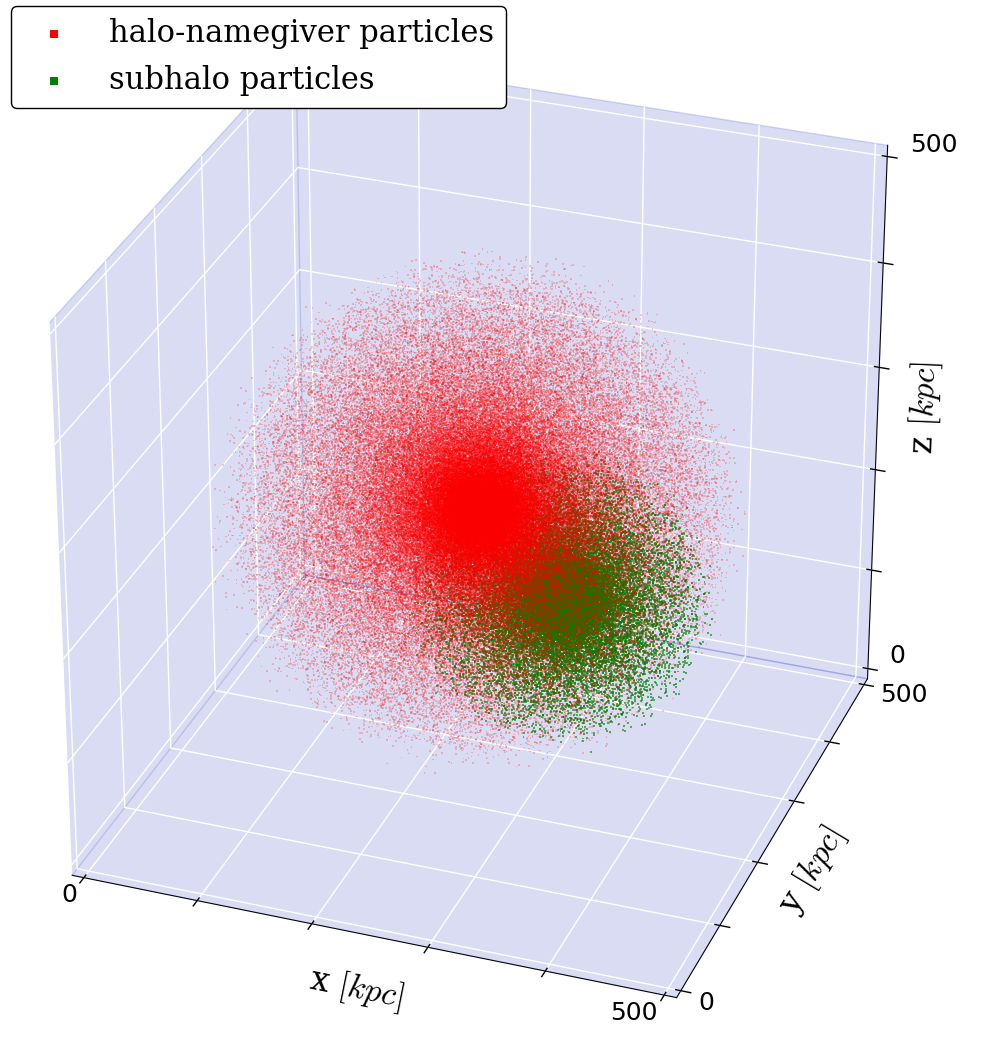
\includegraphics[height=\textwidth]{images/dice-two/dice-two-original-plot.png}}%
		\caption{
			The initial particle distribution of the \dt\ dataset. A smaller halo (subhalo 1) made of 40'000 particles is nested within a bigger halo (halo-namegiver), which contains 200'000 particles.
		}%
		\label{fig:dice_two_origin}
	\endminipage%\hspace{.1cm}
	\hspace*{\fill}
	%
	\minipage[t]{0.497\textwidth}
		\centering
		\fbox{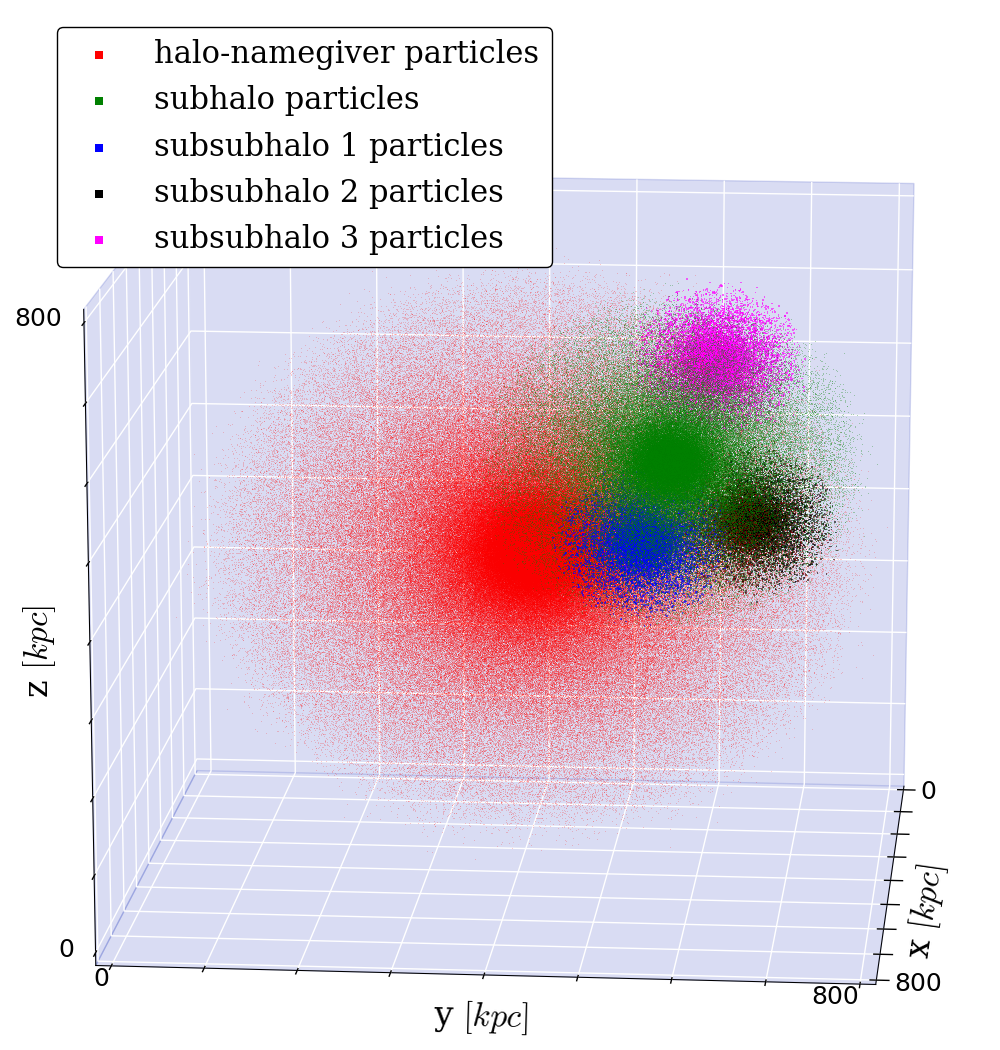
\includegraphics[height=\textwidth, keepaspectratio]{images/dice-sub/dice-sub-original-plot.png}}%
		\caption{
			The initial particle distribution of the \ds\ dataset. 3 small halos (subsubhalo 1-3), made of 20'000 particles, are around a bigger halo (subhalo 1), which contains 200'000 particles. These four structures are then enveloped by an even bigger halo (halo-namegiver), made of 1'000'000 particles.
		}%
		\label{fig:dice_sub_origin}
	\endminipage\hspace*{\fill} 
\end{figure}


%=======================
% DICE SUB
%=======================

The second test case created with \dice, the \ds\ dataset, consists of a halo made of 200'000 particles that has three subhalos, each containing 20'000 particles, following close Kepler orbits around it.
Then this composite structure is enveloped by an even bigger halo with 1'000'000 particles.
The purpose of this dataset is mainly to demonstrate the particle unbinding on a multi-levelled structure hierarchy.
The initial particle distribution is shown in figure \ref{fig:dice_sub_origin}.


%=======================
% COSMO
%=======================

The third dataset, named \cosmo, is a cosmological simulation, aiming to simulate very (physically) large structures and their formation over a long time interval. 
As such, it differs in multiple aspects to the previous two.
Firstly, the particles are described with comoving coordinates to account for the expansion of the Universe.
The computational domain is a cube (``\emph{box}'') of fixed length 1 that contains all the particles.
The physical coordinates of the particles at a certain time can then be computed with respect to the expansion scale factor at that time, thus implementing the expansion of the Universe without need to actually resize the box or move the particles at each time step solely because of the expansion.
Secondly, the simulation uses periodic boundary conditions. 
This means that if a particle would pass a surface of the box, it is reintroduced at the opposite surface.
The usage of periodic boundary conditions allows to simulate an infinite Universe by considering only a part of it and interpreting this part as representative of the entire Universe.
%This idea is justified by the cosmological principle, which states that at very large scales, the Universe is homogeneous and isotropic.
%``Large scales'' in this case are $\sim 100$ Mpc.
%Furthermore, by using periodic boundary conditions, the structures within the box are treated as if they weren't isolated, but influenced by structures outside the box.



The \cosmo\ dataset consists of $128^{3}$ $(\approx 2\cdot10^6)$ dark matter particles at redshift $z=0$ with the Hubble constant $H_0 = 70.4$ and density parameters $\Omega_m = 0.272$ and $\Omega_\Lambda=0.728$
\footnote{
	The density parameter of some cosmological component $i$ is defined as $\Omega_i  = \frac{\rho_i}{\rho_{crit}}$, where $\rho_i$ is its density and  $\rho_{crit}$ is defined as $\rho_{crit} = \frac{3 H^2}{8\pi G}$, where $H$ is the Hubble parameter and $G$ is the gravitational constant.
}.
The density threshold for clump finding was chosen to be 80 times the cosmological critical density $\rho_{crit}$  and the saddle threshold for halos was set to $200\rho_{crit}$.
Only halos with more that 10 particles were kept.
The particle distribution is shown in figure \ref{fig:cosmo_origin}.







\begin{figure}[!htb]
	\centering
	\fbox{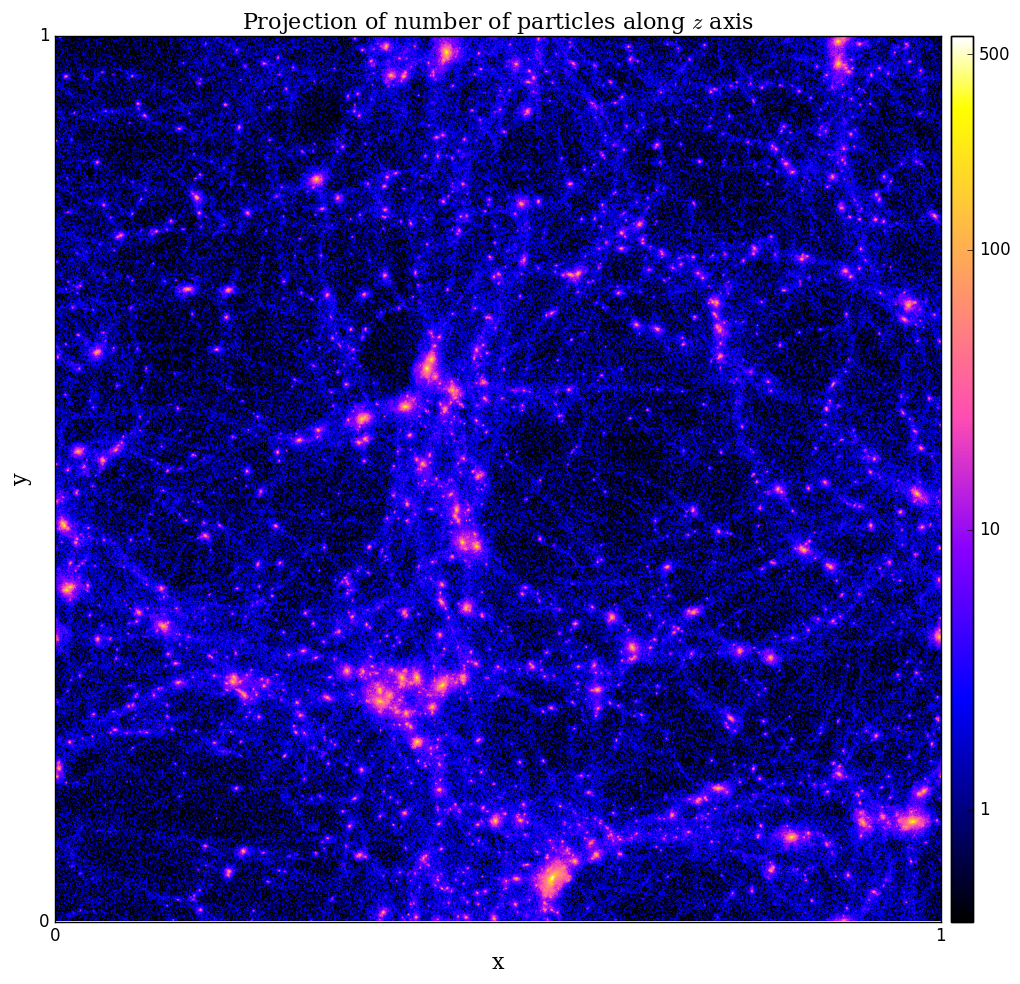
\includegraphics[width = .8\textwidth ]{images/cosmo/cos-part2map-npart.png}}%
	\caption{
		The particle distribution of the \cosmo\ dataset.
		It is a cosmological simulation of $128^3$ dark matter particles at redshift $z=0$ with $H_0 = 70.4$ and density parameters $\Omega_m = 0.272$ and $\Omega_\Lambda=0.728$.
	}%
	\label{fig:cosmo_origin}
\end{figure}

